


\section*{The Quadratic Parent Function}

The quadratic parent function is the \gap{simplest} function that has a quadratic term.

\begin{center}
    \begin{tcolorbox}[width=5in]
        The quadratic \gap{parent function} is written
        \[
            f(x) = x^2
        \]
    \end{tcolorbox}
\end{center}




\myBlankExample{2.5in}{
    Using an $x$-$y$ table,
    sketch the graph of the quadratic parent function,
    $f(x) = x^2$.
}




The graph of the quadratic parent function is shown below.
It looks like a letter \gap{\sffamily\bfseries U}.
(It is similar to but not as ``sharp'' as the absolute value parent function.)
You should be able to quickly sketch this graph in homework or on a test.

\begin{center}
    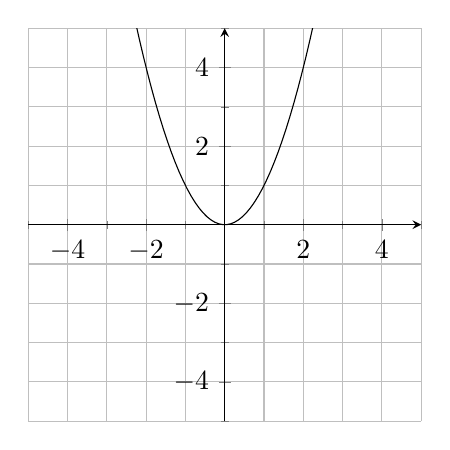
\begin{tikzpicture}
        \begin{axis}[
            width=3in,
            grid=both,
            axis x line = middle,axis y line = middle,
            axis equal image,
            xtick distance = 2, ytick distance = 2,
            xmin = -5, xmax = 5,
            ymin = -5, ymax = 5,
            minor tick num = 1,
            ]
            \addplot[
                no marks,
                mark size = 0.1cm,
                samples=100,
                ] expression { x^2 };
        \end{axis}
    \end{tikzpicture}
\end{center}


For any input, $x$ (positive, zero, or negative), the output $y$ is positive (or zero). 
You can see this, because the graph is completely {\bfseries\itshape above} the $x$-axis,
which means the $y$ values of all the points on the curve are positive (or zero).

\begin{myConceptSteps}{To sketch the graph of the quadratic parent function\dots}
    \myStep{origin}{Draw a dot at the origin: $(0,0)$. This is the \gap{vertex}.}
    \myStep{right dot}{
        Draw a dot at the point \gap{$(1,1)$}.
    }
    \myStep{left dot}{
        Draw a dot at the point \gap{$(-1,1)$}.
    }
    \myStep{fill in}{
        Fill in the curve so that is smoothly passes through the \gap{three dots}.
    }
\end{myConceptSteps}


\myBlankExample{3in}{
    Sketch the graph of the quadratic parent function,
    $f(x) = x^2$.
}
